\section{Design of C-=-1}
\label{language-design}

C-=-1 was designed as a compiled, low-level, non-garbage-collected programming language, similar to C, C++ or Rust.
What diffirentiates C-=-1 are its two founding principles: all code is executable at compile-time and support rich metaprogramming.
The primary purpose of the language was to research how these ideas influence software written in it \cite{grabski2022compilation}.

\subsection{Type system}

\subsection{Attributes and metaprogramming}

\section{Design of the compiler}
\label{compiler-design}

CTFE First apporach was created during implementation of the first compiler for the C-=-1 language\cite{grabski2022compilation}.
CTFE First compiler has four major components: Frontend, Interpreter, Compiler Interface and Backend.
Figure \ref{CTFE-first-compiler-structure} contains a diagram with an overview of how these pieces interact with eachother, during the compilaton process.
Frontend, described in chapter \ref{frontend}, parses the code in the compiled language and constructs its intermidaite representation, using interpreter's data structures.
It is used to analyze both user code and the Compiler Interface.
After the intermidiate representation is constructed, it is passed on to the Interpreter, which was described in chapter \ref{interpreter}.
Compiler Interface intermidiate representation is then executed, using the user program as data. 
This step converts the semantic model of the program into the backends intermidiate language.
This process has been further explained in chapter \ref{compiler-interface}.
Finaly the Backend generates the executable file.

\begin{figure}
	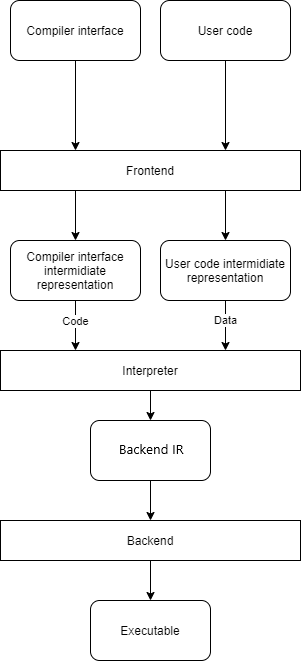
\includegraphics[height=10cm]{pictures/compiler-structure.png}
	\caption{CTFE First compiler structure}
	\label{CTFE-first-compiler-structure}
\end{figure}

\subsection{Frontend}
\label{frontend}

In the CTFE First approach, frontend serves the same role of constructing the programs intermidiate representation, as in conventional compilers \cite{puntambekar:compiler_design}.
The major difference lays in the data structures used to represent the program.

\subsection{Interpreter}
\label{interpreter}

In CTFE First, interpreter is the heart of the compiler.
It executes the Compiler-Interface which translates the intermidiate representation into the backend's assembly and serves as what is sometimes called the 'middle-end' of the compiler\cite{hsu2021llvm}.
To do it, it must be able to treat the program's intermidiate representation both as code and data.


\subsection{Compiler Interface} 
\label{compiler-interface}

Compiler Interface translates the program's intermidaite representation into the backend's assembly language.
This component is interpreted during compilation.
What stands out about CTFE First is that this part of the compiler can thus be written in the target language, during Stage 0 of the compiler bootstrapping process, as was the case for the C-=-1 compiler\cite{puntambekar:compiler_design, novillo2007gcc, grabski2022compilation}.

Compiler Interface is a regular code package that contains a function marked as the Compiler Interface Entry-point.
That procedure must accept a set of modules to be compiled and a Compilation Context that is used to generate the Backends assembly.
The module descriptors that are passed to the Compiler Interface are built by the frontend, as can be seen in figure \ref{CTFE-first-compiler-structure}.

After the Compiler Interface has finished generating backend assembly, the Compiler Backend is invoked to generate the binary executable.
\subsection{Backend}
\label{backend}

CTFE First does not put any additional requierments on compiler backend.
When using this pattern, an out-of-the-box backend library, can be used, as was the case with C-=-1 compiler.

The backend code must be invokable from within the interpreted program in the target language.
Depending on how the interpreter was designed, this can represent a significant undertaking.
Compiler backends are large and for the Compiler Interface to take advantage of them fully, they must be fully available.
This means exposing each function and type within the library, to the interpreted code.
These bindings could feasibly be generated automatically \cite{marshalling_auto_generation}, but this tehnique was not used when implementing C-=-1 compiler.
